\documentclass[a4paper,twoside,11pt,twocolumn]{article}
\usepackage{a4wide,graphicx,fancyhdr,amsmath,amssymb,float,longtable,chronology,caption,subcaption}
\usepackage{algorithmic}
\usepackage{hyperref}
\usepackage{url}

%----------------------- Macros and Definitions --------------------------

\setlength\headheight{20pt}
\addtolength\topmargin{-10pt}
\addtolength\footskip{20pt}

\newcommand{\N}{\mathbb{N}}
\newcommand{\ch}{\mathcal{CH}}
\everymath{\displaystyle}
\newcommand{\solution}[1]{\noindent{\bf Solution to Exercise #1:}}
\newcommand{\scg}{Simulation in Computer Graphics}

\fancypagestyle{plain}{%
	\fancyhf{}
	\fancyhead[LO,RE]{\sffamily\bfseries\large Technische Universiteit Eindhoven}
	\fancyhead[RO,LE]{\sffamily\bfseries\large 2IV15 \scg}
	\fancyfoot[LO,RE]{\sffamily\bfseries\large Department of Mathematics and Computer Science}
	\fancyfoot[RO,LE]{\sffamily\bfseries\thepage}
	\renewcommand{\headrulewidth}{0pt}
	\renewcommand{\footrulewidth}{0pt}
}

\pagestyle{fancy}
\fancyhf{}
\fancyhead[RO,LE]{\sffamily\bfseries\large Technische Universiteit Eindhoven}
\fancyhead[LO,RE]{\sffamily\bfseries\large 2IV15 Simulation in Computer Graphics}
\fancyfoot[LO,RE]{\sffamily\bfseries\large Department of Mathematics and Computer Science}
\fancyfoot[RO,LE]{\sffamily\bfseries\thepage}
\renewcommand{\headrulewidth}{1pt}
\renewcommand{\footrulewidth}{0pt}

%-------------------------------- Title ----------------------------------

\title{\sffamily\bfseries 2IV15 \scg\ - Project 1}
\author{Arno Tiemersma \qquad Student number: 0716959 \\{\tt a.w.g.tiemersma@student.tue.nl}\\ \\Mart Pluijmaekers \qquad Student number: 0753117 \\{\tt m.h.l.pluijmaekers@student.tue.nl}}

\date{\today}

%--------------------------------- Text ----------------------------------

\begin{document}
\maketitle
%\tableofcontents
%\newpage
\section{Introduction}
This paper describes our implementation of a fluid simulator based on papers by Jos Stam \cite{url:stam1, url:stam2}. It supports interaction with the fluid, interaction between the fluid and rigid bodies and interaction between the fluid and a particle system. This text will focus on the changes we made to the skeleton code, and will not describe the skeleton code fully.

\section{Advection and Projection}
The fluid is modeled as a regular grid, having a fluid density and a fluid velocity at the cell center. Both the advection functions and the projection function we implemented follow the methods described in \cite{url:stam1} and \cite{url:stam2}. A short summary of our implementation is given below.

\subsection{Advection}
The density advection function models the fluid densities as a number of particles that are backtraced linearly in time. Using this method the density value in the middle of a grid cell at time $t$ can be calculated by interpolating the densities of the cells that surround the backtraced particle in $t-dt$. Calculating the densities this way is straightforward compared to tracing the particles from the cell centers and then converting the particles back to grid values. 

The velocity advection function is implemented in the same way, but extended for two dimensions.

\subsection{Projection}
The projection function ensures that the velocity field conserves mass. According to the Hodge decomposition, every velocity field is the sum of a mass conserving field and a gradient field. These two fields can be separated by solving the Poisson equation as described in \cite{url:stam2}. This results in a sparse system that can be solved using Gauss-Seidel relaxation. The \texttt{project()} function is called twice during the calculation of one time step, since the advection routine behaves more accurately when the velocity field conserves mass. 

\section{Vorticity Confinement}
Due to the numerical dissipation, small turbulences in the simulated fluid are damped out. Vorticity confinement is a technique that adds these small scale turbulences back to the simulation.
 
The implementation of our vorticity confinement function is based on \cite{fedkiw}. It works by adding small-scale 'rolls' in places where they would physically occur, by looking at the vorticity $\omega$ \[ \mathbf{\omega} = \nabla \times \mathbf{u} \] as a function of the vector field $\mathbf{u}$, which normally provides the small scale turbulence. The idea is to add back the damped out vortices. This is done by calculating normalized vorticity location vectors \textbf{N},  \[\mathbf{\eta} = \nabla|\omega| \]\[ \mathbf{N} = \frac{\mathbf{\eta}}{|\mathbf{\eta}|} \] that indicate where higher vorticity concentrations are located. These are then used to calculate the force of the vortex \[ \mathbf{f_{conf}} = \epsilon\cdot h\cdot(\mathbf{N} \times \mathbf{\omega}) \] where $\epsilon > 0$ determines the amount of detail added back, and spacial discretization $h$ is used to make sure that the correct solution is obtained independent of the mesh resolution.

A result of this simulation is shown in Figure \ref{fig:fluid}. With the grid sizes at which we simulated the fluid and the values we used for $\epsilon$, differences in the simulations with and without vorticity confinement were hard to see.

\begin{figure}[H]
	\centering
	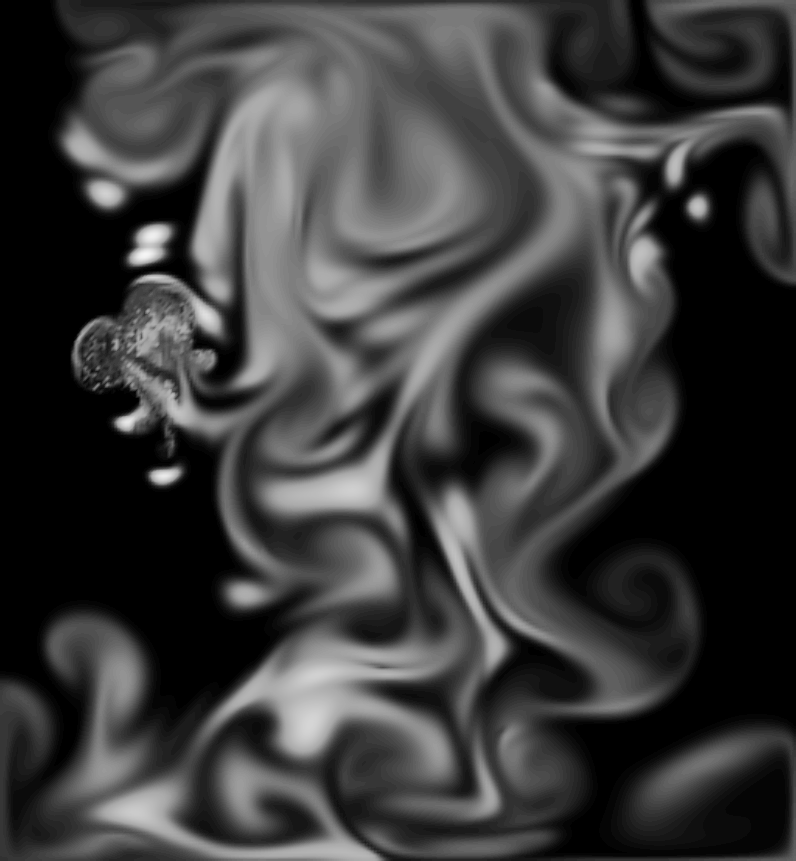
\includegraphics[width=0.45\textwidth]{Fluid}
	\caption{Simulated fluid}
	\label{fig:fluid}
\end{figure}

\section{Particles and Fluids}
We had to slightly adapt the particle system to be able to simulate the effect of the fluid flow. During the force accumulation, the force applied by the velocity field is calculated as a function of the relative speed of the particle compared to the particle's discretized position in the velocity field \[ \mathbf{F} = \mathbf{m\frac{v}{dt}}. \] Taking this force into account the particle system will follow the fluid streams as shown in Figure \ref{fig:particles}.

\begin{figure}[H]
	\centering
	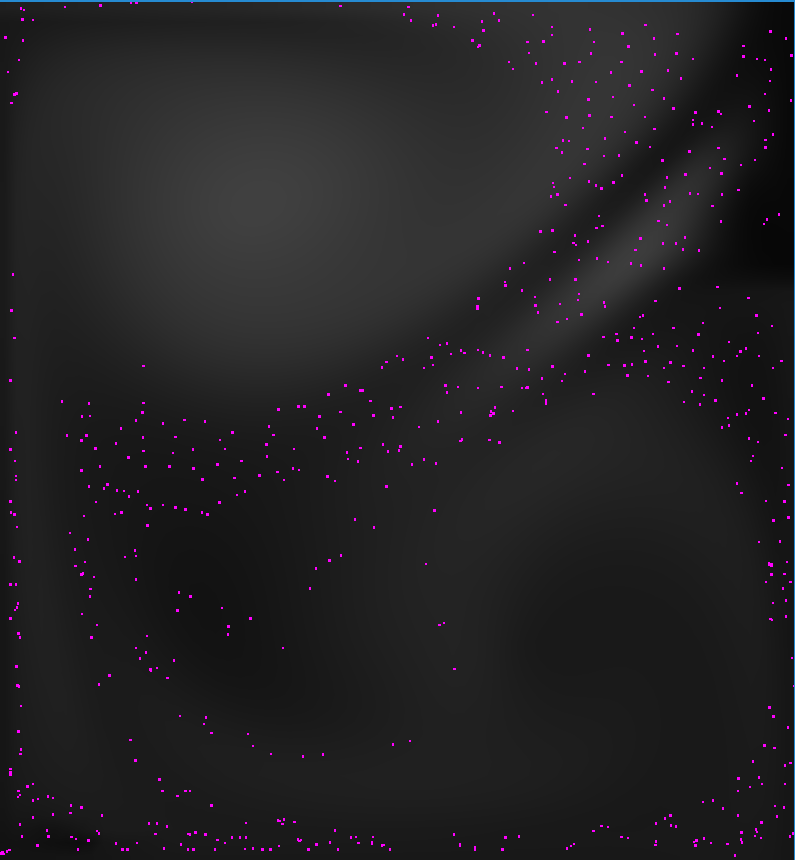
\includegraphics[width=0.45\textwidth]{particles}
	\caption{Particles overlayed on top of the fluid simulation}
	\label{fig:particles}
\end{figure}

For solving the particle system we used the Runge-Kutta 4 solver we implemented during Lab 1, since that method gives the most stable and accurate results. Using this particle system allowed us to simulate both uncoupled, unconstrained particles that affected by the fluid and a primitive cloth simulation using particles connected by springs as shown in Figure \ref{fig:cloth}.

\begin{figure}[H]
	\centering
	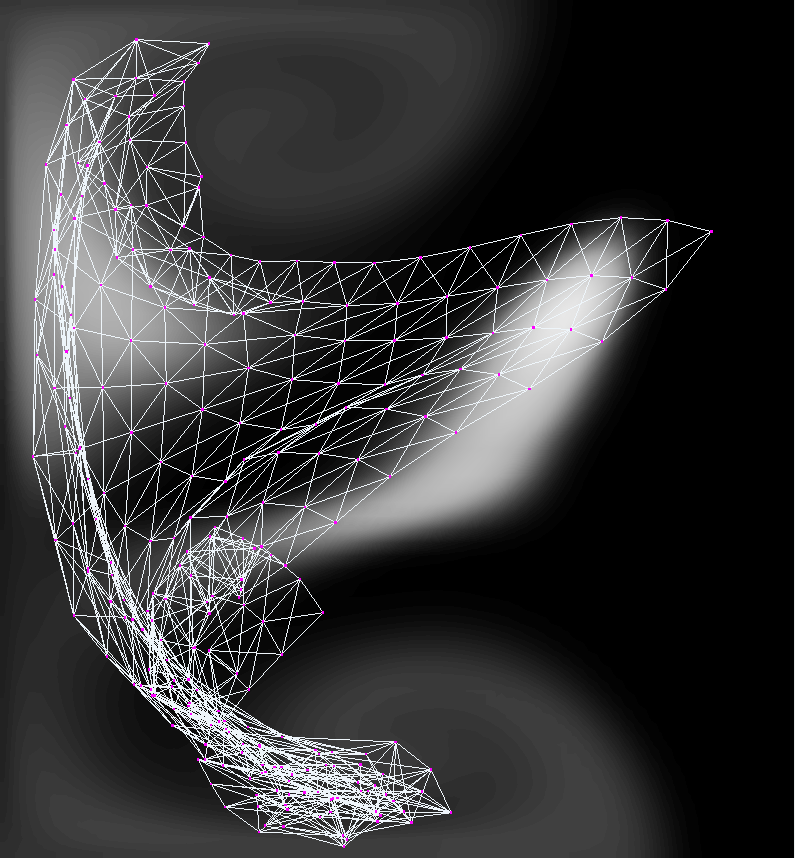
\includegraphics[width=0.45\textwidth]{cloth}
	\caption{Cloth affected by the fluid}
	\label{fig:cloth}
\end{figure}

These results could be made more physically accurate by interpolating the particle's position instead of rounding it down, but since the current implementation gives visually accurate results we decided to focus on the rest of the implementation.

Using the particle system in combination with the fluid simulation can result in complex, visually pleasing images, such as those shown in this paper.

\section{Rigid Bodies}

\section{Conclusion}
In this paper, we presented a fluid simulator following the methods described in \cite{url:stam1, url:stam2}, with added vorticity confinement, fluid interaction and interaction with rigid bodies and a particle system. There was not much visual difference between the simulation with and without vorticity confinement at the grid sizes and values for $\epsilon$ we experimented with.
The motion of the simulated fluid looks visually accurate, and using the particle system in combination with the fluid simulation can result in interesting and visually pleasing images.
% TODO: add something about rigid bodies


\begin{thebibliography}{9}
	\bibitem{url:stam1}
		Stam, Jos. \emph{''Stable Fluids''} Computer Graphics (SIGGRAPH 1999), ACM, 121-128. \url{http://www.dgp.toronto.edu/people/stam/reality/Research/pdf/ns.pdf}
	\bibitem{url:stam2}
		Stam, Jos. \emph{''Real-Time Fluid Dynamics for Games''} Proceedings of the Game Developer Conference, March 2003. \url{http://www.dgp.toronto.edu/people/stam/reality/Research/pdf/GDC03.pdf}
	\bibitem{fedkiw}
		Fedkiw, R., Stam, J., Jensen, H. \emph{Visual Simulation of Smoke.} Computer Graphics (SIGGRAPH 2001), ACM, 15-22.
	
\end{thebibliography}
\end{document}
